\documentclass[10pt,twocolumn]{article}

\usepackage[margin=1.7cm,columnsep=0.6cm]{geometry}
\usepackage{mathptmx}
\usepackage[T1]{fontenc}
\usepackage{graphicx}
\usepackage{booktabs}
\usepackage{caption}
\usepackage{amsmath}
\usepackage{xcolor}
\usepackage[colorlinks=true,linkcolor=blue!50!black,citecolor=blue!50!black,urlcolor=blue!50!black]{hyperref}
\usepackage{titlesec}
\usepackage{enumitem}

\setlength{\parskip}{2pt}
\setlength{\abovecaptionskip}{3pt}
\setlength{\belowcaptionskip}{-4pt}
\titlespacing*{\section}{0pt}{6pt}{3pt}
\titlespacing*{\subsection}{0pt}{4pt}{2pt}
\captionsetup{font=small,labelfont=bf}

\newcommand{\tcd}{\ensuremath{\mathrm{TCD}}}

\title{\vspace{-1.2em}\textbf{Evaluating Agentic AI for Supply-Chain Disruption Mitigation}\\
\large A Two-Phase Paired-Simulation Study of a Bounded LLM Agent Against a Classical Heuristic\\
\normalsize\itshape Extended Edition -- with full-grid visuals and a reinforcement-learning follow-up}
\author{\small Yassine Erraji \\[-2pt] \small \texttt{supply-chain-agent-evaluation} -- Full Study, Versions 1 \& 2}
\date{\small August 2026}

\begin{document}
\maketitle
\vspace{-1.6em}

\begin{abstract}
\noindent Can a bounded, tool-using large language model (LLM) agent mitigate supply-chain disruption more effectively than a transparent, cost-minimizing classical heuristic -- and if so, under what conditions? We answer this in two phases, sharing one paired-simulation infrastructure throughout. \textbf{Phase 1} tested one network topology against three disruption severities (300 real, live-API replications) and found the LLM agent losing under Light disruption but winning decisively under Medium/Heavy -- with every one of 300 replications agreeing unanimously (100\%/0\% per profile), a result too clean to trust at face value. Auditing why traced the unanimity to insufficient environmental randomness and a single, low-redundancy topology, not to a genuine effect ceiling. \textbf{Phase 2} redesigned the experiment along exactly the axes the audit implicated: three network topologies crossed with the same three severities (nine cells, 498 replications), plus per-replication randomness in disruption timing, duration, disclosure, and shipment volume. The redesign both validated Phase 1 (the original topology reproduces its original pattern almost exactly) and overturned its implicit generality: \textbf{network topology does not merely scale the LLM's advantage -- it can reverse its sign}, with the highest-redundancy topology favoring the heuristic ever more strongly as severity rises, the opposite of the other two topologies. Across the whole two-phase program, agentic AI shows a real, statistically confirmed advantage for high-stakes disruption response on constrained networks, and a real, equally confirmed disadvantage under low-stakes conditions and high-redundancy networks -- a nuanced, conditional answer, not a universal one. This edition adds the full-grid heatmap and the signal-to-noise validation figure, plus a follow-up section on a reinforcement-learning formulation of the same decision problem.
\end{abstract}

\section{Research Problem}
\label{sec:intro}
Agentic AI -- LLM-based systems that reason, call tools, and act -- is increasingly proposed for operational supply-chain decisions: rerouting, expediting, or cancelling shipments in response to disruption, where a wrong call has directly measurable cost. The claim that ``AI beats the baseline'' rarely survives scrutiny in this domain: mismatched scenarios, cherry-picked examples, or a classical baseline never given a fair, symmetric shot. This study's overarching goal, spanning both phases reported here, is to test that claim rigorously for one narrow, well-defined decision -- \emph{what should happen to a shipment sitting at a node when the surrounding network is disrupted} -- and to answer not just \emph{whether} an agentic policy helps, but \emph{when}: \textbf{under identical disrupted conditions and identical operational constraints, can a bounded LLM policy reduce the incremental cost of disruption more effectively and more robustly than a transparent classical heuristic, and how does that advantage depend on network structure and disruption severity?}

Fairness is operationalized structurally, not asserted: both policies observe identical read-only state, are validated and fall back through the same machinery, and face the same stochastic demand, delay, and disruption realization within a replication. Each policy is scored against its own undisrupted counterfactual, isolating the \emph{incremental} cost of disruption rather than baseline operating cost.

\section{Related Work}
\label{sec:relwork}
\textbf{LLM agents with tools.} ReAct \cite{yao2022react} established the now-standard interleaved reasoning--action--observation loop for LLM agents, later made reliable via structured function calling; Toolformer \cite{schick2023toolformer} showed LLMs can learn \emph{when} to invoke tools rather than merely being prompted to. Our agent follows this lineage: five deterministic, read-only tools, an 8-call budget, temperature 0, and a hard fallback to the classical heuristic on abstention or invalid output.

\textbf{LLM agents in supply chain management.} This is an active, recent direction: InvAgent \cite{invagent2024} applies multi-agent LLMs to inventory management under demand uncertainty; broader surveys \cite{llmscm2025} catalog knowledge-integration and negotiation as dominant use cases; \cite{agenticscm2025} studies autonomous multi-agent consensus across supply-chain roles. This literature consistently flags a verification gap -- agentic LLMs can inherit biases and produce confidently wrong decisions absent explicit checking -- which is precisely why this study reports null and unfavorable results for the agent alongside favorable ones, rather than only the latter.

\textbf{Classical disruption management.} The heuristic baseline sits in a long tradition of cost-minimizing routing and recovery rules under disruption \cite{sheffi2005resilient,christopher2004building}: transparent, auditable, structurally incapable of considering information outside its candidate-route cost estimate. It is not a strawman -- it wins cleanly in both phases under Light disruption, and dominates one topology entirely in Phase 2.

\section{Shared Methodology}
\label{sec:method}
Both phases run on one unmodified simulator: a discrete-time, single-product network (suppliers~$\to$~ports~$\to$~hubs~$\to$~plant) in which a policy intervenes on at most one shipment per decision point with exactly one action -- \texttt{WAIT}, \texttt{REROUTE}, \texttt{EXPEDITE}, or \texttt{ABSTAIN} -- validated by shared rules with a heuristic-then-\texttt{WAIT} fallback on failure.

One random seed drives one \emph{replication}: demand, ordinary transport delay, and (Phase 2 only) disruption realization and shipment volume are drawn entirely before either policy acts. Four cloned branches then run per replication -- \{heuristic, LLM\}~$\times$~\{undisrupted, disrupted\} -- sharing an identical 20-day warm-up snapshot. Per policy $p$, $\tcd_p = J^{\text{disrupted}}_p - J^{\text{undisrupted}}_p$ ($J$ sums transport, reroute, expedite, holding, backlog, late, and terminal costs); the reported effect is $\Delta = \tcd_{\text{LLM}} - \tcd_{\text{heuristic}}$ ($\Delta<0$ favors the LLM). Pairing removes common-mode noise, since the same random world hits both policies, giving far more power per replication than an unpaired design.

\section{Phase 1: Initial Evaluation}
\label{sec:phase1}
Phase 1 tested one network (5 nodes, 6 edges, $\sim$3 end-to-end routes) against three fixed disruption severities -- a partial-capacity cut (Light), a full 7-day port closure (Medium), and a 3-week closure plus alternate-route congestion (Heavy) -- 100 live-API replications each, 300 total.

\begin{table}[t]
\centering
\small
\begin{tabular}{@{}lrrr@{}}
\toprule
Severity & Mean $\Delta$ & 95\% CI & LLM win \\
\midrule
Light  & $+992$ & [967, 1018] & 0\% \\
Medium & $-3{,}911$ & [$-$4011, $-$3811] & 100\% \\
Heavy  & $-74{,}490$ & [$-$75919, $-$73061] & 100\% \\
\bottomrule
\end{tabular}
\caption{Phase 1: mean $\Delta$ and 95\% CI, $n=100$/severity. Every one of the 300 replications agreed unanimously with every other in its profile.}
\label{tab:v1}
\end{table}

\textbf{Headline result.} The LLM agent loses under Light disruption but wins decisively under Medium and Heavy (Table~\ref{tab:v1}) -- a clean, seemingly interpretable severity gradient. \textbf{The problem}: within every profile, all 100 replications agreed with each other exactly (100\%/0\%), never once split. Auditing why traced this to three compounding, fixable design properties, not a genuine effect ceiling: (i) the shipment release schedule was fully deterministic, exactly 40 units every day; (ii) the disruption's timing, duration, and disclosure were fully known in advance; (iii) the network offered only $\sim$3 routes -- not enough structure for a close call to ever arise. Quantitatively, the mean $|\Delta|$ was $7.6\times$--$10.2\times$ larger than the between-replication standard deviation of $\Delta$ in every profile: the experiment could not generate a world where the effect and the noise were remotely comparable in scale, so unanimity was close to guaranteed by construction, not by an overwhelming true effect. This motivated Phase 2.

\section{Phase 2: Topology-Generalized Evaluation}
\label{sec:phase2}
Phase 2 targets the audit's three causes directly, without altering the shared simulator, action space, validator, cost model, or pairing logic (Section~\ref{sec:method}). \textbf{Topology}: three tiers -- Compact (4 nodes/4 edges/0 non-emergency reroutes), Standard (Phase 1's original network, byte-identical), and Extended (10 nodes/16 edges/7 structurally distinct non-emergency routes, confirmed by betweenness centrality) -- crossed independently with the same three severities. \textbf{Randomness}: disruption start day, duration, and disclosure delay are now sampled per replication rather than fixed (a zero-uncertainty template provably reproduces Phase 1 bit-for-bit); shipment quantity is sampled per release on Compact/Extended (Standard keeps Phase 1's fixed 40 units by design, as an unmodified behavioral anchor). Extended's severity scenarios target \texttt{hub\_1} rather than \texttt{port\_primary}, since centrality analysis showed the latter is no longer that tier's structural chokepoint once seven alternate routes exist.

Nine cells result, each an independently-run configuration. Compact and Extended run 33 replications/cell; Standard runs Phase 1's original 100/cell as the reference column. All nine were calibrated (3 replications each) before the full run, which then executed live against the OpenAI API: 498 replications, $\sim$14{,}700 LLM calls, $\sim$4.5\,h wall-clock across three concurrent per-topology processes, all nine completing without error.

\begin{table}[t]
\centering
\small
\begin{tabular}{@{}llrrr@{}}
\toprule
Topology & Severity & Mean $\Delta$ & 95\% CI & LLM win \\
\midrule
Compact  & Light  & $+935$ & [814, 1055]      & 0\% \\
Compact  & Medium & $-1{,}436$ & [$-$2210, $-$663] & \textbf{75.8\%} \\
Compact  & Heavy  & $-56{,}915$ & [$-$68896, $-$44934] & 100\% \\
Standard & Light  & $+921$ & [857, 985]        & 0\% \\
Standard & Medium & $-4{,}192$ & [$-$4682, $-$3702] & 100\% \\
Standard & Heavy  & $-111{,}850$ & [$-$122960, $-$100741] & 100\% \\
Extended & Light  & $+1{,}636$ & [1451, 1820]    & 0\% \\
Extended & Medium & $+5{,}176$ & [4536, 5817]    & 0\% \\
Extended & Heavy  & $+22{,}114$ & [17950, 26279]  & 0\% \\
\bottomrule
\end{tabular}
\caption{Phase 2: mean $\Delta$ and 95\% CI on all nine cells. $n=33$ (Compact/Extended), $n=100$ (Standard). Every CI excludes zero.}
\label{tab:v2}
\end{table}

\textbf{Validation.} Standard~$\times$~Medium is Phase~1's original configuration, re-run unmodified at Phase 2 scale: LLM wins 100\% of 100 replications, matching Phase 1's original pattern almost exactly (compare Table~\ref{tab:v1}'s Medium row) -- the shared infrastructure did not silently break. \textbf{Headline result}: Compact and Standard reproduce Phase 1's shape, the LLM's advantage growing with severity. \textbf{Extended inverts it} -- the heuristic's advantage grows with severity instead, winning every replication at every severity (Figure~\ref{fig:interaction}). Topology is not a magnitude dial on a fixed direction of effect; it can flip which policy is favored as conditions worsen. This is visible at a glance across the whole grid in Figure~\ref{fig:heatmap}: no cell is hatched, since every 95\% CI excludes zero, so every color shown is a real effect.

\begin{figure}[t]
\centering
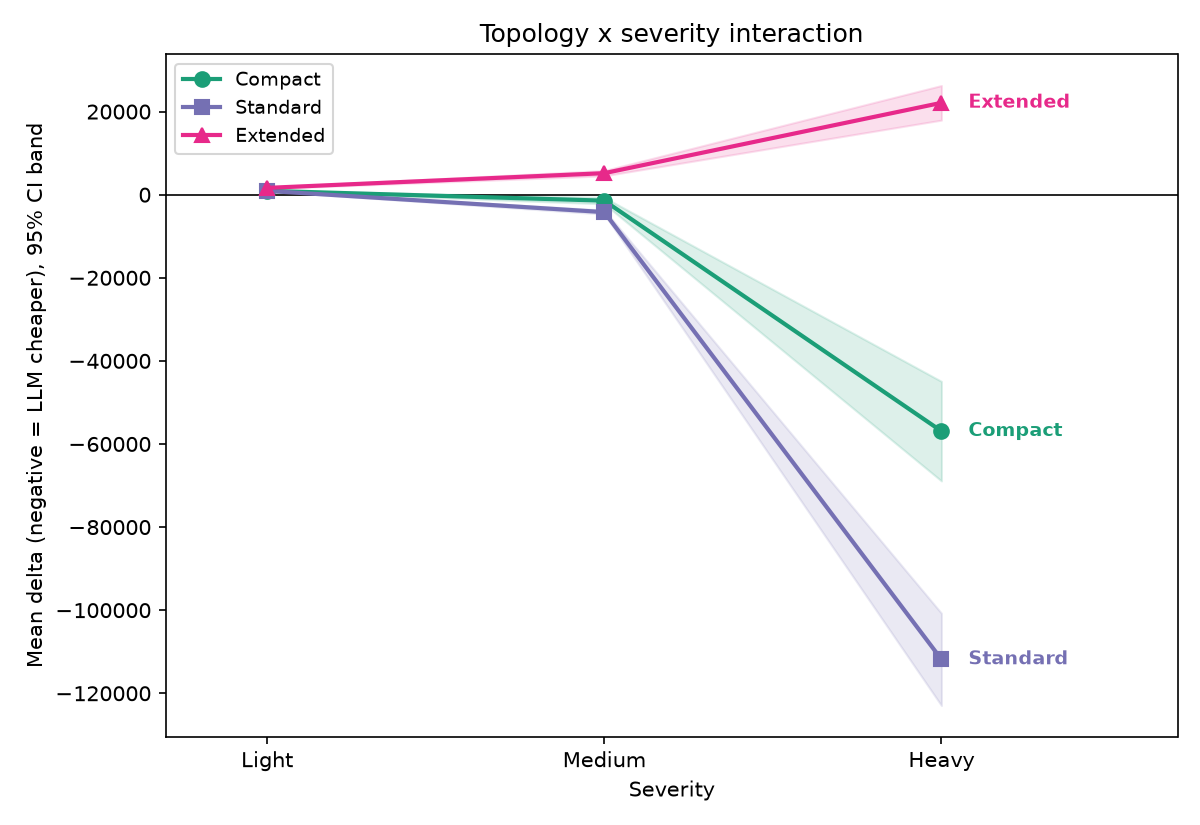
\includegraphics[width=\linewidth]{../analysis/plots/v2_grid_full/grid/12_topology_severity_interaction.png}
\caption{Phase 2: mean $\Delta$ vs.\ severity, one line per topology (signed-sqrt axis; bands are 95\% CI). Compact/Standard diverge negative (LLM-favorable); Extended diverges positive (heuristic-favorable).}
\label{fig:interaction}
\end{figure}

Separately, Compact~$\times$~Medium becomes the first cell in either phase to land away from unanimity (75.8\% LLM, 24.2\% heuristic) -- direct evidence the redesign produces genuine per-replication variation. Consistent with this, the signal-to-noise ratio $|\overline{\Delta}|/\mathrm{sd}(\Delta)$ sits at 0.6$\times$--3.0$\times$ across all nine Phase 2 cells, against the $7.6\times$--$10.2\times$ recomputed identically on Phase 1's real runs (Figure~\ref{fig:snr}) -- the audited root cause is measurably fixed, not merely asserted fixed.

\begin{figure}[t]
\centering
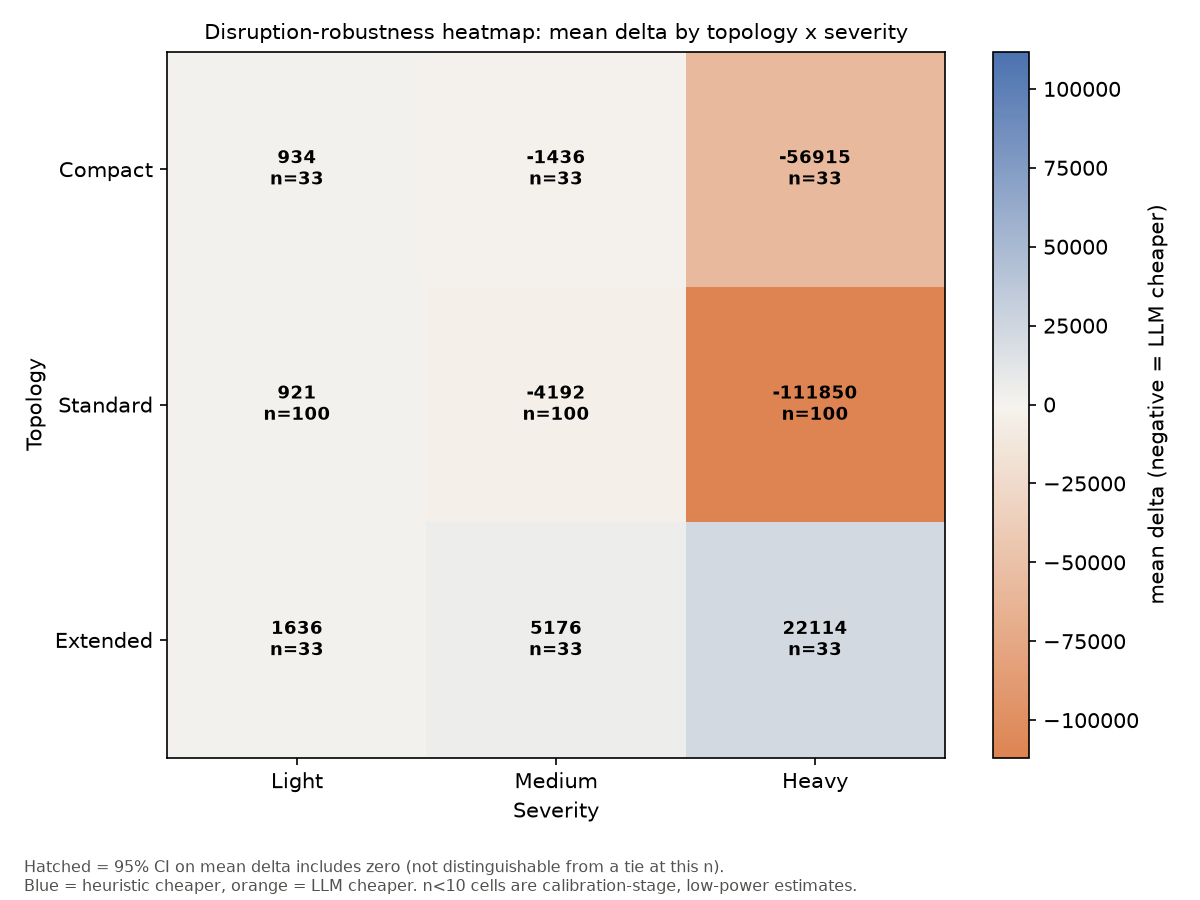
\includegraphics[width=\linewidth]{../analysis/plots/v2_grid_full/grid/08_disruption_robustness_heatmap.png}
\caption{Phase 2: mean $\Delta$ across the full grid (diverging color; orange = LLM-favorable, blue = heuristic-favorable). Every cell's effect is statistically real at its sample size.}
\label{fig:heatmap}
\end{figure}

\section{Discussion: Synthesis Across Both Phases}
Combining 798 replications across two phases and four network configurations, the study's answer to its research question is conditional, not universal. \textbf{Pros of the agentic policy}: substantially larger cost reduction under severe disruption on constrained-to-moderate topologies (up to $-111{,}850$ mean $\Delta$); the only policy to ever produce a genuinely mixed, non-unanimous outcome (Compact~$\times$~Medium), suggesting situational judgment rather than a fixed rule; this advantage replicated independently across two separate live-API runs on the same network (Phase 1 and Phase 2's Standard column). \textbf{Cons}: consistently worse under Light disruption in every configuration tested (\texttt{WAIT} is usually already optimal, and reasoning/tool-call overhead buys nothing); worse at every severity on the highest-redundancy topology; real monetary cost and $\sim$2.6\,s of live-API latency per decision, against a free, instant, deterministic heuristic evaluation. A plausible mechanism for the Extended reversal: the heuristic exhaustively scores every candidate route by estimated cost and never has to judge which of many plausible options is worth pursuing, while a bounded agent (max 8 tool calls) reasons under genuinely higher ambiguity as the option count grows -- plausible, not proven (see Limitations).

\begin{figure}[t]
\centering
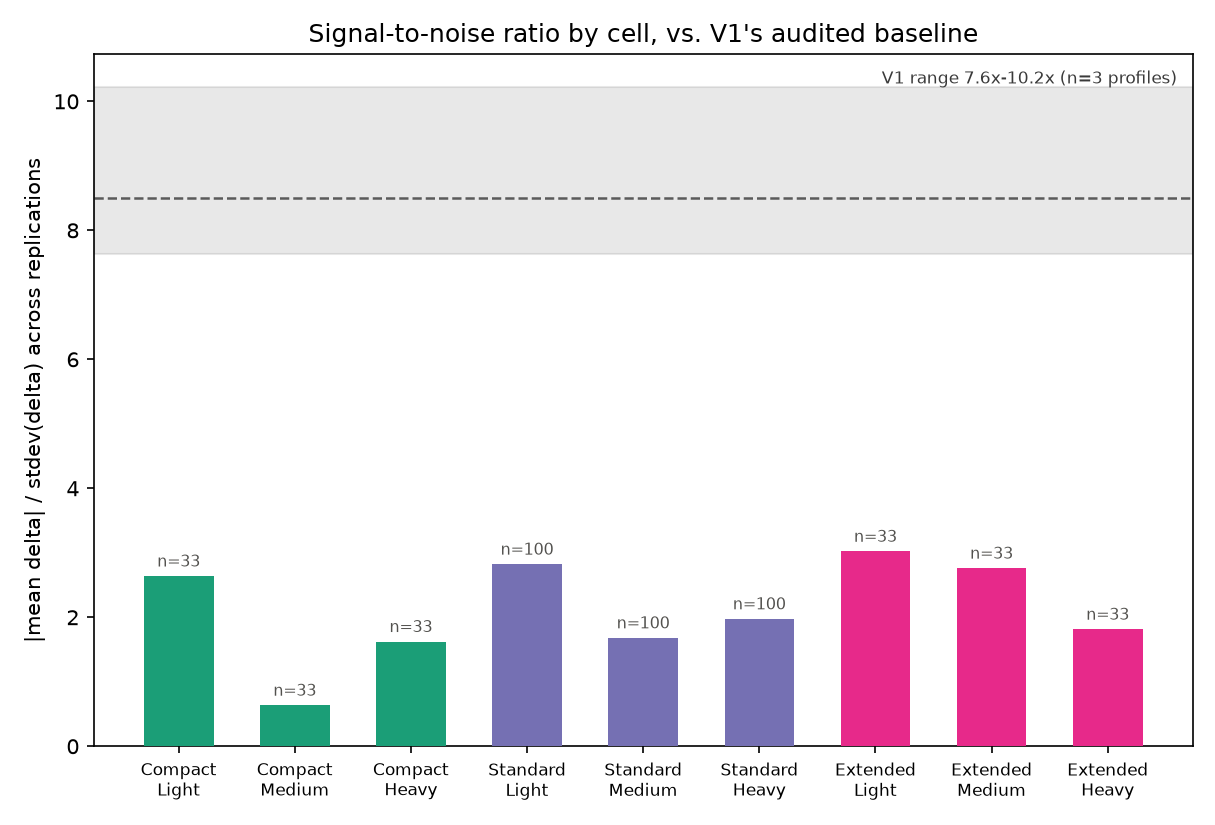
\includegraphics[width=\linewidth]{../analysis/plots/v2_grid_full/grid/14_signal_to_noise_by_cell.png}
\caption{$|\overline{\Delta}|/\mathrm{sd}(\Delta)$ per Phase 2 cell against Phase 1's real, identically-computed baseline (shaded band). Every Phase 2 cell sits well under Phase 1's 7.6$\times$--10.2$\times$.}
\label{fig:snr}
\end{figure}

\section{Limitations and Nuance}
\label{sec:limits}
Four nuances qualify the combined findings. \textbf{(1)} Extended's severity scenarios target \texttt{hub\_1}, not \texttt{port\_primary} -- justified (Section~\ref{sec:phase2}), but it entangles the reversal with \emph{which node} is attacked, not topology redundancy alone. \textbf{(2)} Standard's shipment quantity stays fixed across both phases by design, while Compact/Extended draw real variance -- an acknowledged confound on any comparison involving Standard specifically. \textbf{(3)} Phase 2's 33 replications/cell is real, CI-confirmed power, but less than Phase 1's 100/profile; Compact~$\times$~Medium's split could plausibly shift with more replications. \textbf{(4)} Both phases use one model, one temperature, one prompt template, and one narrow decision (single-shipment routing) -- this is a finding about one policy design tested twice, not a general claim about agentic AI in logistics.

\section{Follow-up: A Reinforcement-Learning Formulation}
\label{sec:rl}
Both policies studied here are, in a precise sense, \emph{not learned}: the heuristic is a fixed rule, and the LLM agent's behavior comes from pre-trained general reasoning plus a prompt, not from experience inside this environment. A natural follow-up is to add a third arm that \emph{is} learned: a reinforcement-learning (RL) policy trained directly against the simulator's own state, action, and reward structure.

The formulation is close to already sitting in the codebase. \textbf{State}: the same read-only \texttt{DecisionObservation} both existing policies already receive -- shipment facts, destination and shock context, current plan, candidate routes. \textbf{Action}: the same four-choice space, \texttt{WAIT}/\texttt{REROUTE}/\texttt{EXPEDITE}/\texttt{ABSTAIN}, already shared and validated identically. \textbf{Reward}: the negative of the same daily cost terms ($J$) already accumulated for $\tcd$, either shaped per-day (dense) or given once at episode end as $-\tcd$ (sparse, but exactly the metric this study already optimizes for by construction). Because the simulator's transitions are already deterministic and the event tapes are already fully pre-generated and replayable, an RL agent can be trained across thousands of simulated episodes at effectively zero marginal cost -- a sharply different economics from the LLM arm, where every decision is a paid, $\sim$2.6\,s API call, and one of the more interesting comparisons this study does not yet make: cost-per-decision at training time versus cost-per-decision at deployment time.

What it could add beyond the current two-policy comparison: \textbf{(i) an empirical reference point} -- if a policy free to learn via trial and error over many episodes converges to a similar decision boundary as the heuristic or the LLM, that is independent evidence neither current policy is leaving much value on the table; if it instead discovers materially different behavior (for instance, rerouting proactively before a shock is fully disclosed, something neither current policy is built to do), that is itself a finding. \textbf{(ii) a way to separate environment from agent} in the Extended-topology reversal reported above: if a trained RL policy \emph{also} reverses on Extended, that argues the reversal is a structural property of the decision problem itself, independent of which agent is solving it; if an RL policy does not reverse there, that argues the LLM's specific bounded-reasoning behavior, not the environment, is responsible -- a distinction Section~\ref{sec:limits} could not resolve with the two policies tested here.

This is not a free upgrade. An RL policy loses the heuristic's auditability and the LLM's natural-language reasoning trace -- its decision boundary is a learned function, not a rule a person can read. Reward shaping is itself a research decision with failure modes (a dense per-day reward can encourage short-sighted behavior; a sparse terminal reward is harder to learn from). And a policy trained on one topology/severity distribution is not guaranteed to generalize to another without deliberately training across the full nine-cell grid, which reintroduces, at training time, exactly the topology-dependence this study's headline result already shows matters.

\section{Conclusion}
Two phases, one shared paired-simulation infrastructure, and 798 live-API replications give a conditional but well-evidenced answer to whether agentic AI mitigates supply-chain disruption better than a classical heuristic: \textbf{it depends on both disruption severity and network structure, and the dependence on structure is not monotonic in the way Phase 1 alone would have suggested.} The agent's advantage is real and large on constrained-to-moderate networks under severe disruption; the heuristic's advantage is equally real, and grows rather than shrinks, on the most redundant network tested. Phase 1's audit-driven redesign into Phase 2 is itself part of the finding: an experiment that cannot produce anything but unanimous agreement is not evidence of robustness, and the discipline of building an environment able to disagree with itself is what surfaced the topology-reversal result in the first place. Near-term, future work should decouple Extended's shock target from its topology, equalize shipment-volume variance across tiers, and extend the demand-side and supplier-side shock types already built but not yet run at grid scale; longer-term, the reinforcement-learning formulation above offers a way to test whether either policy studied here is close to a ceiling, or whether the topology-reversal finding is about the environment rather than the agent.

\begin{thebibliography}{9}
\footnotesize
\bibitem{yao2022react} S.~Yao et al., ``ReAct: Synergizing Reasoning and Acting in Language Models,'' \emph{arXiv:2210.03629}, 2022.
\bibitem{schick2023toolformer} T.~Schick et al., ``Toolformer: Language Models Can Teach Themselves to Use Tools,'' \emph{arXiv:2302.04761}, 2023.
\bibitem{invagent2024} Y.~Song et al., ``InvAgent: A Large Language Model based Multi-Agent System for Inventory Management in Supply Chains,'' \emph{arXiv:2407.11384}, 2024.
\bibitem{llmscm2025} ``Large Language Models for Supply Chain Management,'' \emph{arXiv:2505.18597}, 2025.
\bibitem{agenticscm2025} ``Agentic LLMs in the Supply Chain: Towards Autonomous Multi-Agent Consensus-Seeking,'' \emph{International Journal of Production Research}, 2025.
\bibitem{sheffi2005resilient} Y.~Sheffi, \emph{The Resilient Enterprise: Overcoming Vulnerability for Competitive Advantage}. MIT Press, 2005.
\bibitem{christopher2004building} M.~Christopher and H.~Peck, ``Building the Resilient Supply Chain,'' \emph{International Journal of Logistics Management}, 15(2), 2004.
\end{thebibliography}

\end{document}
